\documentclass[11pt,preprint, authoryear]{elsarticle}

\usepackage{lmodern}
%%%% My spacing
\usepackage{setspace}
\setstretch{1.2}
\DeclareMathSizes{12}{14}{10}{10}

% Wrap around which gives all figures included the [H] command, or places it "here". This can be tedious to code in Rmarkdown.
\usepackage{float}
\let\origfigure\figure
\let\endorigfigure\endfigure
\renewenvironment{figure}[1][2] {
    \expandafter\origfigure\expandafter[H]
} {
    \endorigfigure
}

\let\origtable\table
\let\endorigtable\endtable
\renewenvironment{table}[1][2] {
    \expandafter\origtable\expandafter[H]
} {
    \endorigtable
}


\usepackage{ifxetex,ifluatex}
\usepackage{fixltx2e} % provides \textsubscript
\ifnum 0\ifxetex 1\fi\ifluatex 1\fi=0 % if pdftex
  \usepackage[T1]{fontenc}
  \usepackage[utf8]{inputenc}
\else % if luatex or xelatex
  \ifxetex
    \usepackage{mathspec}
    \usepackage{xltxtra,xunicode}
  \else
    \usepackage{fontspec}
  \fi
  \defaultfontfeatures{Mapping=tex-text,Scale=MatchLowercase}
  \newcommand{\euro}{€}
\fi

\usepackage{amssymb, amsmath, amsthm, amsfonts}

\def\bibsection{\section*{References}} %%% Make "References" appear before bibliography


\usepackage[round]{natbib}

\usepackage{longtable}
\usepackage[margin=2.3cm,bottom=2cm,top=2.5cm, includefoot]{geometry}
\usepackage{fancyhdr}
\usepackage[bottom, hang, flushmargin]{footmisc}
\usepackage{graphicx}
\numberwithin{equation}{section}
\numberwithin{figure}{section}
\numberwithin{table}{section}
\setlength{\parindent}{0cm}
\setlength{\parskip}{1.3ex plus 0.5ex minus 0.3ex}
\usepackage{textcomp}
\renewcommand{\headrulewidth}{0.2pt}
\renewcommand{\footrulewidth}{0.3pt}

\usepackage{array}
\newcolumntype{x}[1]{>{\centering\arraybackslash\hspace{0pt}}p{#1}}

%%%%  Remove the "preprint submitted to" part. Don't worry about this either, it just looks better without it:
\makeatletter
\def\ps@pprintTitle{%
  \let\@oddhead\@empty
  \let\@evenhead\@empty
  \let\@oddfoot\@empty
  \let\@evenfoot\@oddfoot
}
\makeatother

 \def\tightlist{} % This allows for subbullets!

\usepackage{hyperref}
\hypersetup{breaklinks=true,
            bookmarks=true,
            colorlinks=true,
            citecolor=blue,
            urlcolor=blue,
            linkcolor=blue,
            pdfborder={0 0 0}}


% The following packages allow huxtable to work:
\usepackage{siunitx}
\usepackage{multirow}
\usepackage{hhline}
\usepackage{calc}
\usepackage{tabularx}
\usepackage{booktabs}
\usepackage{caption}


\newenvironment{columns}[1][]{}{}

\newenvironment{column}[1]{\begin{minipage}{#1}\ignorespaces}{%
\end{minipage}
\ifhmode\unskip\fi
\aftergroup\useignorespacesandallpars}

\def\useignorespacesandallpars#1\ignorespaces\fi{%
#1\fi\ignorespacesandallpars}

\makeatletter
\def\ignorespacesandallpars{%
  \@ifnextchar\par
    {\expandafter\ignorespacesandallpars\@gobble}%
    {}%
}
\makeatother

\newenvironment{CSLReferences}[2]{%
}

\urlstyle{same}  % don't use monospace font for urls
\setlength{\parindent}{0pt}
\setlength{\parskip}{6pt plus 2pt minus 1pt}
\setlength{\emergencystretch}{3em}  % prevent overfull lines
\setcounter{secnumdepth}{5}

%%% Use protect on footnotes to avoid problems with footnotes in titles
\let\rmarkdownfootnote\footnote%
\def\footnote{\protect\rmarkdownfootnote}
\IfFileExists{upquote.sty}{\usepackage{upquote}}{}

%%% Include extra packages specified by user

%%% Hard setting column skips for reports - this ensures greater consistency and control over the length settings in the document.
%% page layout
%% paragraphs
\setlength{\baselineskip}{12pt plus 0pt minus 0pt}
\setlength{\parskip}{12pt plus 0pt minus 0pt}
\setlength{\parindent}{0pt plus 0pt minus 0pt}
%% floats
\setlength{\floatsep}{12pt plus 0 pt minus 0pt}
\setlength{\textfloatsep}{20pt plus 0pt minus 0pt}
\setlength{\intextsep}{14pt plus 0pt minus 0pt}
\setlength{\dbltextfloatsep}{20pt plus 0pt minus 0pt}
\setlength{\dblfloatsep}{14pt plus 0pt minus 0pt}
%% maths
\setlength{\abovedisplayskip}{12pt plus 0pt minus 0pt}
\setlength{\belowdisplayskip}{12pt plus 0pt minus 0pt}
%% lists
\setlength{\topsep}{10pt plus 0pt minus 0pt}
\setlength{\partopsep}{3pt plus 0pt minus 0pt}
\setlength{\itemsep}{5pt plus 0pt minus 0pt}
\setlength{\labelsep}{8mm plus 0mm minus 0mm}
\setlength{\parsep}{\the\parskip}
\setlength{\listparindent}{\the\parindent}
%% verbatim
\setlength{\fboxsep}{5pt plus 0pt minus 0pt}



\begin{document}



\begin{frontmatter}  %

\title{Question 1}

% Set to FALSE if wanting to remove title (for submission)




\author[Add1]{Peter Meihuizen}
\ead{21831041@sun.az.za}





\address[Add1]{Stellenbosch Univerity, South Africa}



\vspace{1cm}


\begin{keyword}
\footnotesize{
Multivariate GARCH \sep Kalman Filter \sep Copula \\
\vspace{0.3cm}
}
\footnotesize{
\textit{JEL classification} L250 \sep L100
}
\end{keyword}



\vspace{0.5cm}

\end{frontmatter}

\setcounter{footnote}{0}



%________________________
% Header and Footers
%%%%%%%%%%%%%%%%%%%%%%%%%%%%%%%%%
\pagestyle{fancy}
\chead{}
\rhead{}
\lfoot{}
\rfoot{\footnotesize Page \thepage}
\lhead{}
%\rfoot{\footnotesize Page \thepage } % "e.g. Page 2"
\cfoot{}

%\setlength\headheight{30pt}
%%%%%%%%%%%%%%%%%%%%%%%%%%%%%%%%%
%________________________

\headsep 35pt % So that header does not go over title




\hypertarget{introduction}{%
\section{\texorpdfstring{Introduction
\label{Introduction}}{Introduction }}\label{introduction}}

For this question I am looking at how different continents were affected
by Covid-19.

\hypertarget{analysis}{%
\section{\texorpdfstring{Analysis
\label{Analysis}}{Analysis }}\label{analysis}}

Ok so firstly I need to import the data.

I want to compare how Covid affected African countries relative to other
continents. In order to do this I'm going to compare various COVID-19
statistics over 6 month intervals for every continent. Therefore I will
divide the times period into 5 periods: 2020-01, 2020-07, 2021-01,
2021-07 and 2022-01. I will give the mean value for each of these
continents over each 6 month period.

In order to do this I need to build a function which calculates the mean
value for a particular country over this a particular 6 month period.

I want to look at the mean value for total\_cases\_by\_million for each
country so I'll use the function calculate the mean for each country
based on each period.

Ok so this function is giving me errors and is not working so I'm going
to try simplify it to calculate the mean\_total cases for each country
in that particular period, first I'm going to add a period column to the
main data frame indicating the 5 different periods.

Now I generate the bargraphs showings the growing rates of the average
cases, hospitalisations, deaths and vaccinations.

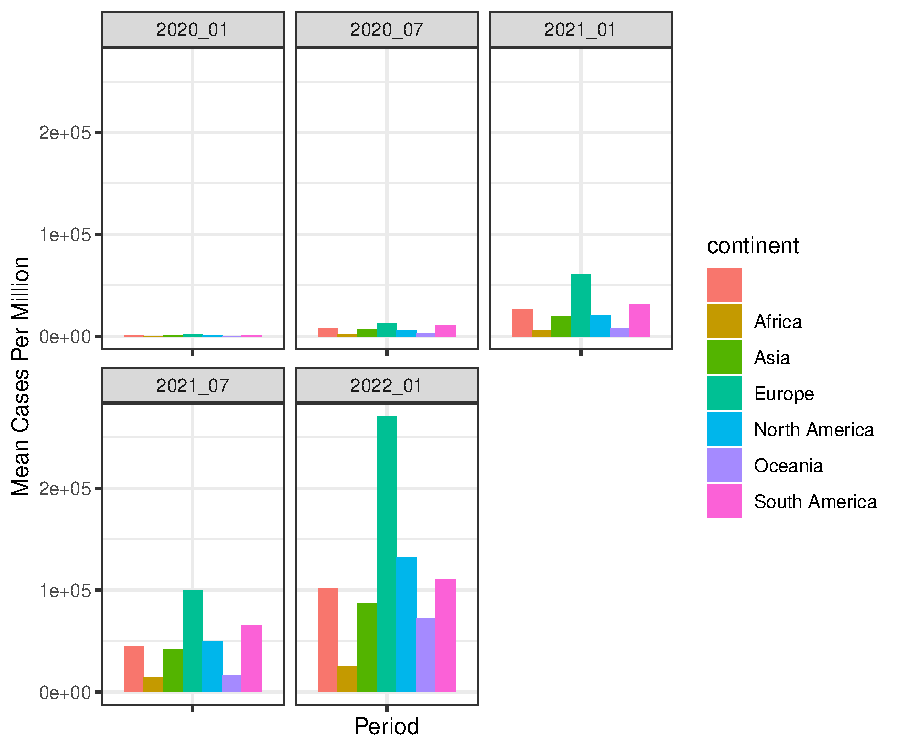
\includegraphics{Question_1_files/figure-latex/unnamed-chunk-3-1.pdf}
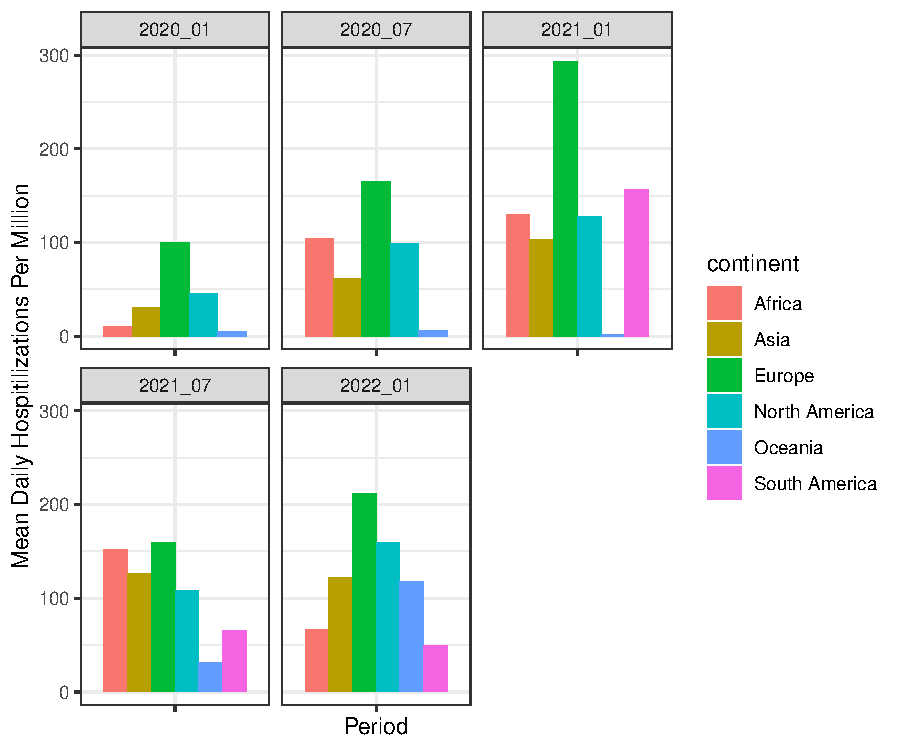
\includegraphics{Question_1_files/figure-latex/unnamed-chunk-3-2.pdf}
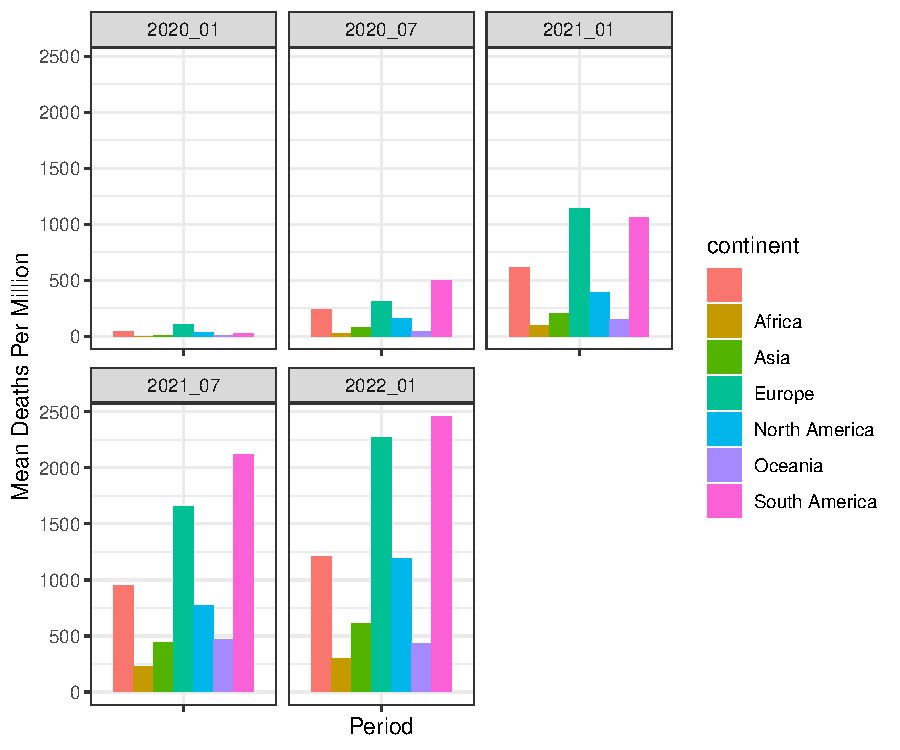
\includegraphics{Question_1_files/figure-latex/unnamed-chunk-3-3.pdf}
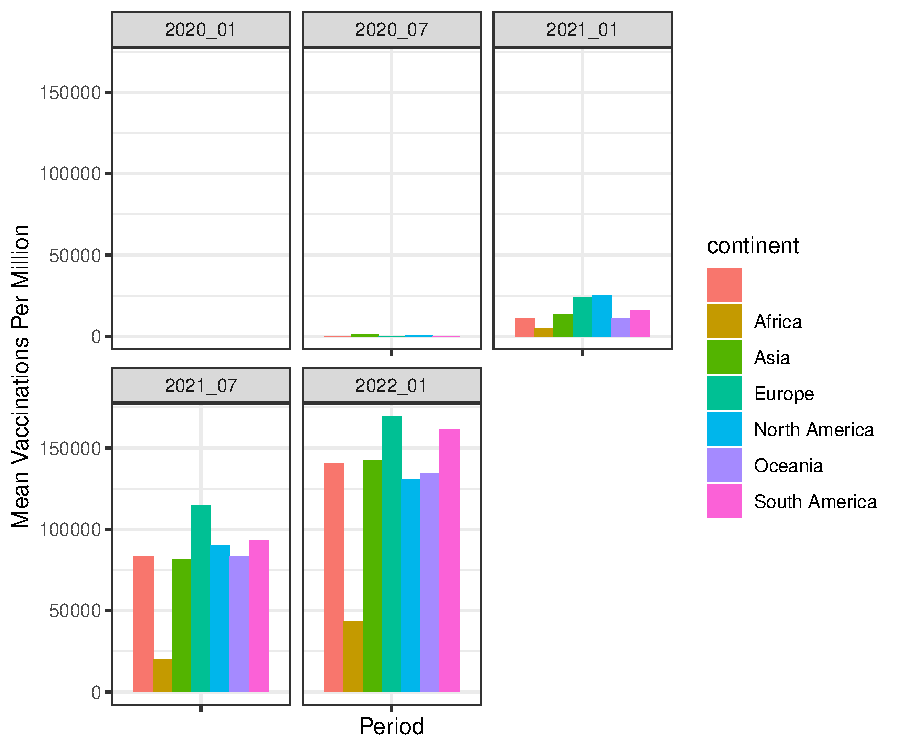
\includegraphics{Question_1_files/figure-latex/unnamed-chunk-3-4.pdf}

Ok so as can be seen in the results Africa is the least affected by
Covid on all accounts. Of all the continents it has the lowest number of
cases, hospitalisations, deaths and vaccinations per million of every
continent. It appears the more developed continents, Europe and North
America are the most significantly affected.

For the next part of my analysis I want to look at the correlation
between smoking and hospitalisations to see if countries with an higher
rate of smoking are more likely to be hospitalised. I need to import the
death\_by\_cause data to look at smoking related deaths.

Because Europe was most significantly affected by Covid I want to only
look at European countries to do my comparison, I therefore want to look
at those countries which had the greatest level of lower respiratory
infections as these can cause higher death rates amongst smokers as they
have weaker lungs. Therefore I need to look at the European countries
with the 3 greatest number of average daily hospitalisations and the 3
lowest. I will find the hospitialisations and populations of all
measured European countries.

\begin{verbatim}
## # A tibble: 30 x 3
##    location  mean_hosp mean_pop
##    <chr>         <dbl>    <dbl>
##  1 Bulgaria       469.  6896655
##  2 Serbia         419.  6871547
##  3 Lithuania      362.  2689862
##  4 Romania        326. 19127772
##  5 Hungary        290.  9634162
##  6 France         265. 67422000
##  7 Poland         255. 37797000
##  8 Latvia         231.  1866934
##  9 Croatia        228.  4081657
## 10 Czechia        220. 10724553
## # i 20 more rows
\end{verbatim}

Ok so based on this it shows that the highest daily hospitalisations for
Covid in Europe over the five periods were in Bulgaria, Serbia,
Lithuania, Romania and Hungary whilst the lowest recorded daily
hospitalisations were in Norway, Finland, Iceland, Denmark and the
Netherlands.

Now I need to look at each countries prevalence for smoking by averaging
their respiratory infection deaths form the Deaths\_by\_cause data set.

Now I need to combine these two sets to compare respiratory deaths with
covid hospitalisation and create a respiratoty deaths per population
variable.

Now that I have the average number of Covid hospitalisations and the
number of lower respiratory infection deaths per million of the
population I can create a scatter polt to see if their was any
correlation.

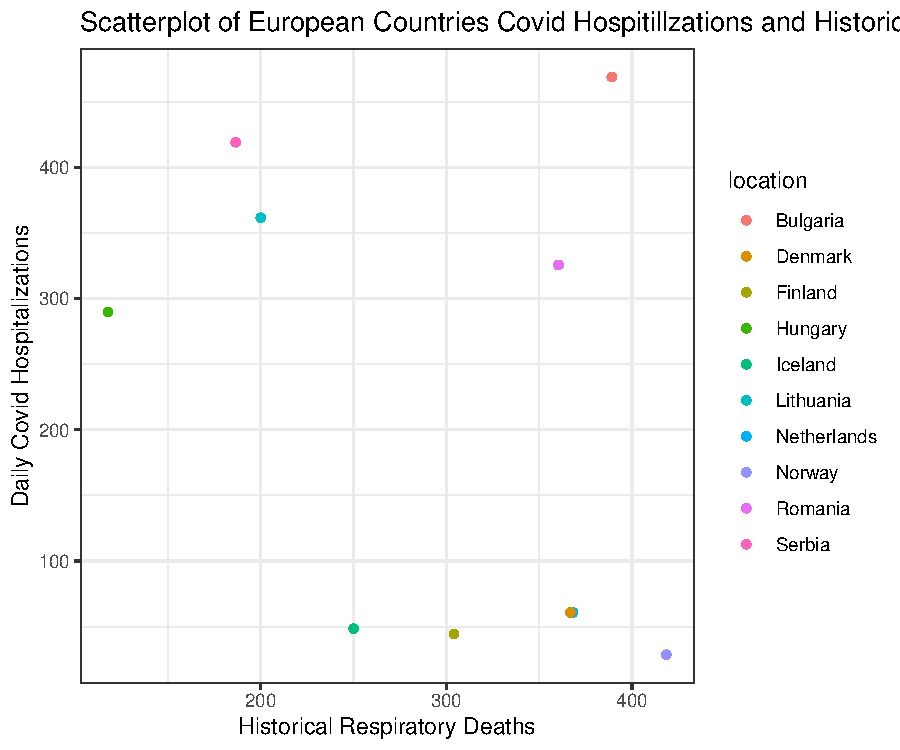
\includegraphics{Question_1_files/figure-latex/unnamed-chunk-8-1.pdf}

\begin{verbatim}
## # A tibble: 10 x 3
##    location    mean_hosp percent_resp_deaths
##    <chr>           <dbl>               <dbl>
##  1 Bulgaria        469.                 389.
##  2 Serbia          419.                 187.
##  3 Lithuania       362.                 200.
##  4 Romania         326.                 360.
##  5 Hungary         290.                 118.
##  6 Netherlands      60.8                368.
##  7 Denmark          60.8                367.
##  8 Iceland          48.5                250.
##  9 Finland          44.3                304.
## 10 Norway           28.6                418.
\end{verbatim}

So as can be seen there is almost no correlation between the historical
respiratory deaths and daily Covid hospitilations for countries in
Europe. This would suggest that countries with historically high levels
of smoking are unlikely to have more or less covid-related
hospitalisations.

For the final part of the question I'm going to look at hospitalisation
numbers and ICU numbers for each continent and see if the one led or
lagged the other. Ok so first I'm going to group the data by continent
and by month.

\begin{verbatim}
## # A tibble: 209 x 4
##    continent year_month cont_hosp cont_ICU
##    <chr>     <chr>          <dbl>    <dbl>
##  1 ""        2020-01          NaN      NaN
##  2 ""        2020-02          NaN      NaN
##  3 ""        2020-03          NaN      NaN
##  4 ""        2020-04          NaN      NaN
##  5 ""        2020-05          NaN      NaN
##  6 ""        2020-06          NaN      NaN
##  7 ""        2020-07          NaN      NaN
##  8 ""        2020-08          NaN      NaN
##  9 ""        2020-09          NaN      NaN
## 10 ""        2020-10          NaN      NaN
## # i 199 more rows
\end{verbatim}

Now I want to plot the data to see if hospitalisations number lead or
lag ICU numbers.

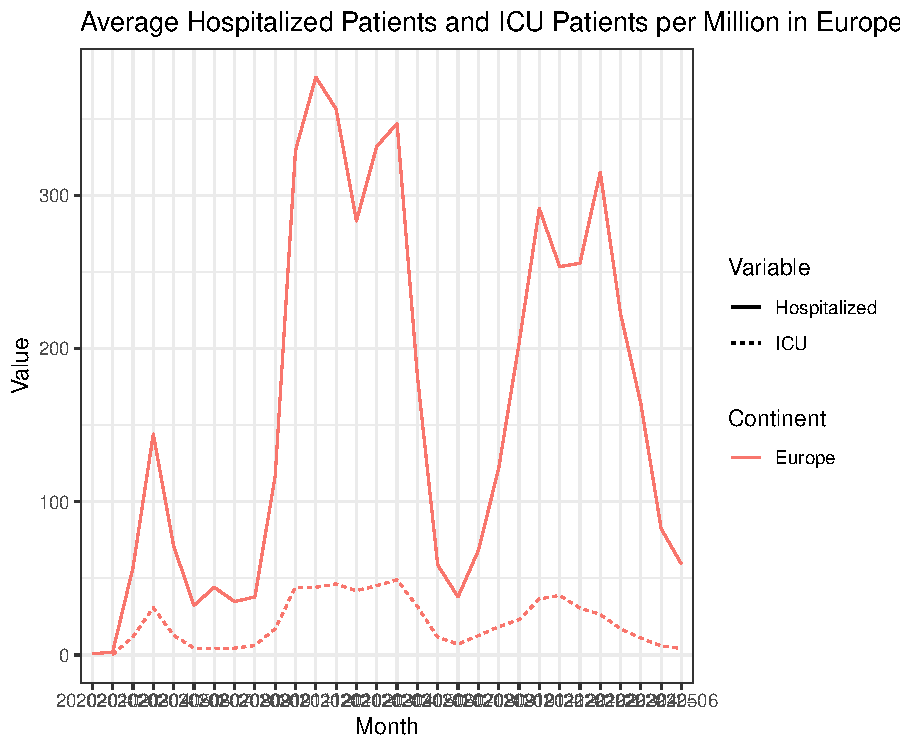
\includegraphics{Question_1_files/figure-latex/unnamed-chunk-10-1.pdf}
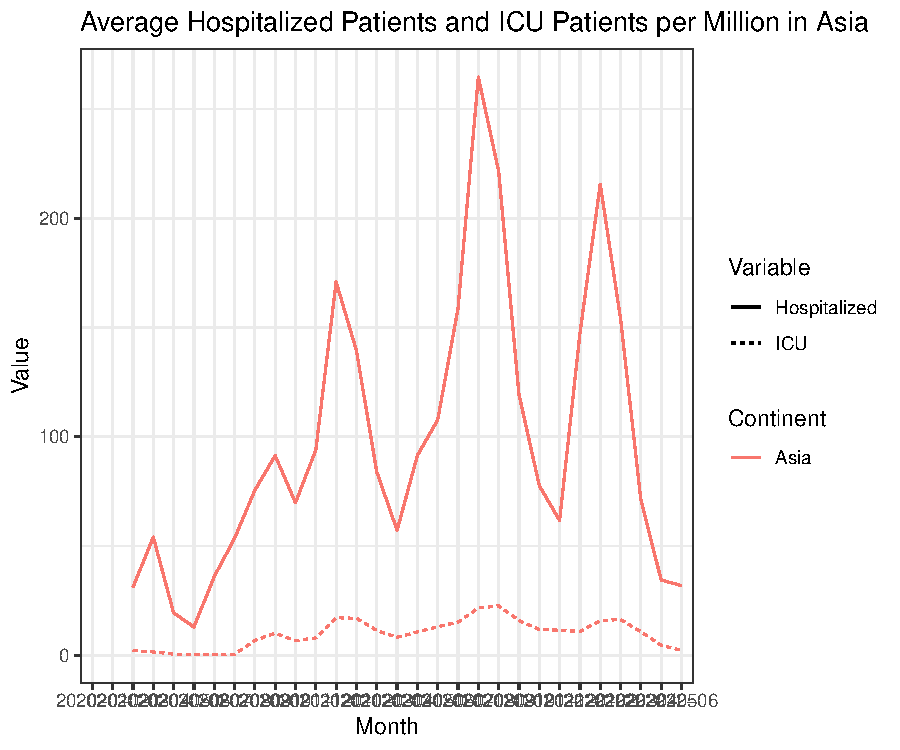
\includegraphics{Question_1_files/figure-latex/unnamed-chunk-10-2.pdf}
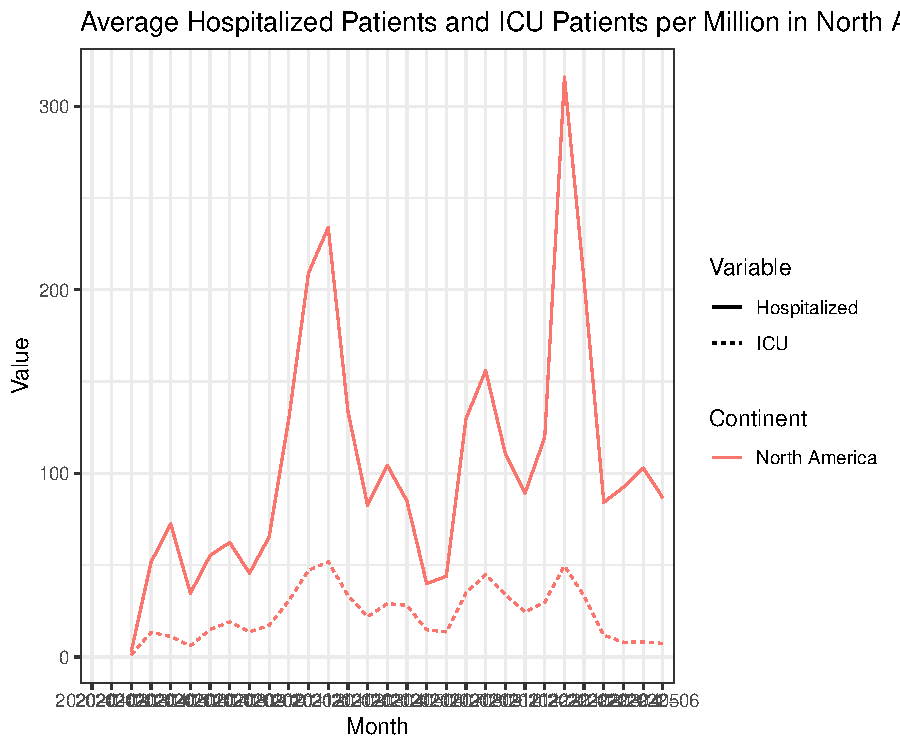
\includegraphics{Question_1_files/figure-latex/unnamed-chunk-10-3.pdf}

Therefore it appears that the level of hospitalizations, which is being
used as a proxy for hospital capacity, coincides with an increase in ICU
admissions for Europe, Asia and North America when looking at the
monthly admissions.

\bibliography{Tex/ref}





\end{document}
